\noindent
\textbf{Inspiração biológica} \\

    O cérebro humano possui um tipo específico de célula que aparentemente não se regenera lentamente como as outras. A estas células são atribuídas a capacidade de pensamento, lembranças e transferência de todo tipo de informações para todo o corpo. Estas células chamadas neurônios estão presentes em quantidades que chegam a aproximadamente 100 bilhões de unidades \cite{anderson1992artificial}.
    O neurônio é dividido em basicamente três partes como mostrado na Figura 1: núcleo, axônio e dendritos, e cada uma delas tem sua atividade bem estipulada. O núcleo é onde ocorre todo o processamento dos sinais elétricos recebidos pelos dendritos que ficam nas extremidades da célula e são transmitidos pelo axônio para o próximo neurônio.

    \begin{figure}[ht]
        \centering
        \label{fig01}
            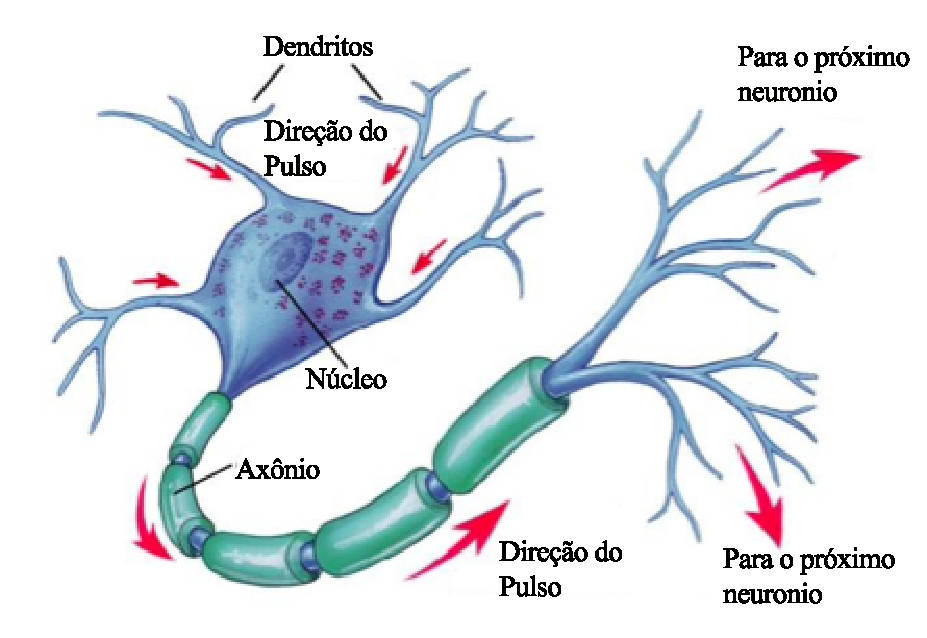
\includegraphics[keepaspectratio=true, scale=0.4]{editaveis/images/neuronio.eps}
        \caption{Representação de neurônio humano}
        Fonte: Adaptado de \cite{marieb2009}
    \end{figure}

    Estes pulsos, ou sinais elétricos, são transmitidos do axônio de um neurônio para os dendritos de um outro neurônio através das fendas sinápticas, ou sinapses como mostrado na Figura 2.

    \begin{figure}[ht]
        \centering
        \label{fig02}
            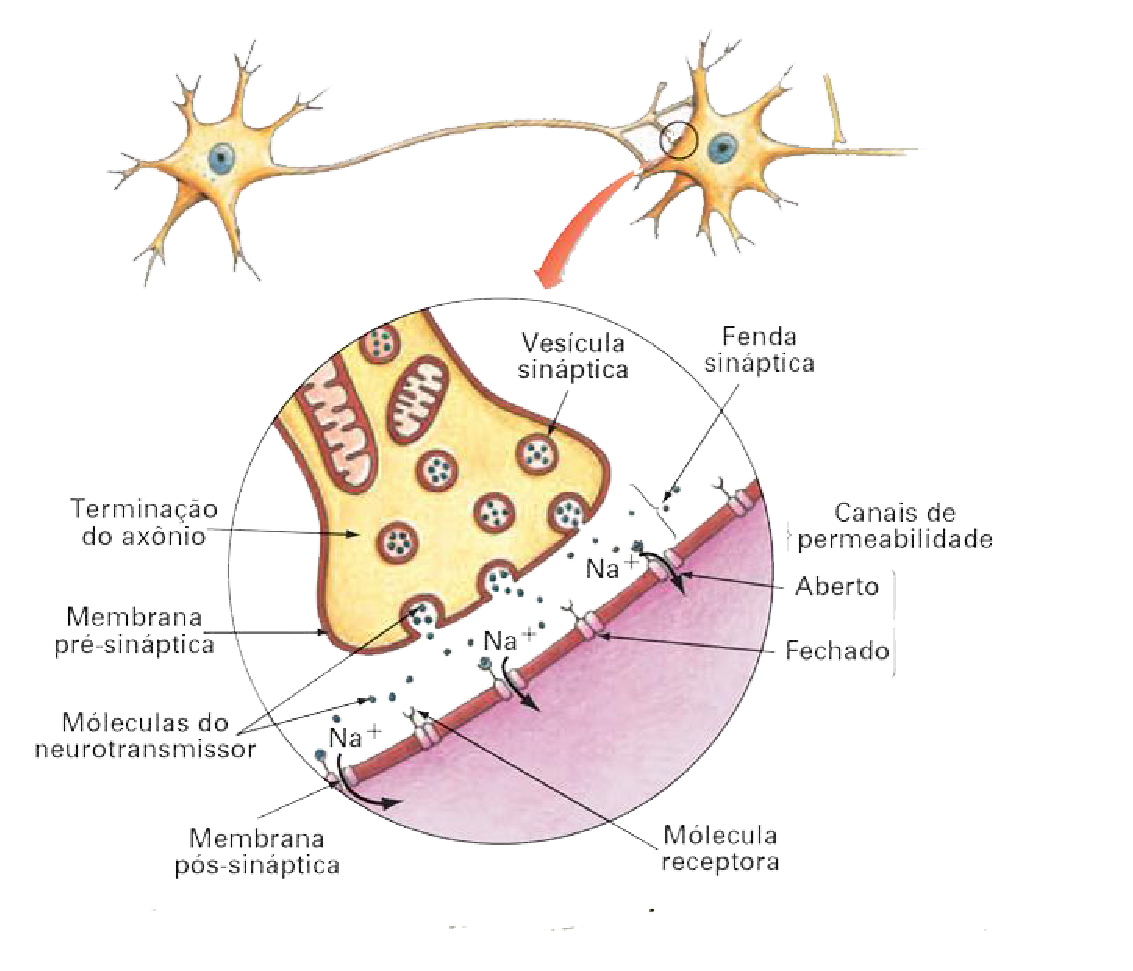
\includegraphics[keepaspectratio=true, scale=0.4]{editaveis/images/sinapse.eps}
        \caption{Representação de uma sinápse.}
        Fonte : Adaptado de \cite{marieb2009}
    \end{figure}

    As sinápses são eventos ativos eletroquimicamente entre as membranas celulares dos neurônios, onde a partir de uma excitação ocorre uma reação química que transmite os sinais de uma célula a outra por intermédio de substâncias chamadas neurotransmissores \cite{marieb2009}.

\noindent
\textbf{Modelagem matemática}
    O neurônio biológico pode ser modelado matematicamente de um modo que inspire a criação de um neurônio artificial a partir dessa divisão. Sendo assim, uma modelagem matemática de um neurônio biológico é \cite{rocha2006}:

    \begin{itemize}
        \item Entrada: São os dendritos, por onde os sinais chegam;
        \item Pesos: São as áreas onde as informações são transferidas de um neurônio para outro,  ou seja, as sinápses;
        \item Soma: É o núcleo do neurônio, onde cada entrada é multiplicada com seu devido peso para que em seguida passe por uma função de transferência, a qual vai gerar os sinais de saída dos axônios;
        \item Função de Transferência: É o potencial necessário para ativação das fendas sinápticas.
        \item Saída: São os axônios do neurônio biológico.
    \end{itemize}

    Dessa maneira, tomando por base este modelo, o desenho de um neurônio artificial é mostrado na Figura 3.

    \begin{figure}[ht]
        \centering
        \label{fig03}
            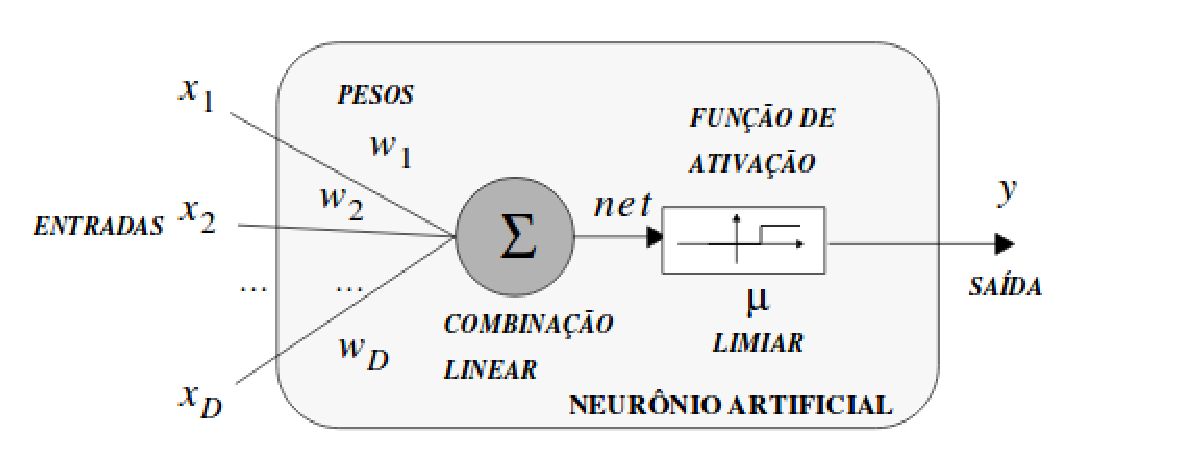
\includegraphics[keepaspectratio=true, scale=0.27]{editaveis/images/modeloNeuronio.eps}
        \caption{Representação matemática do neurônio.}
        Fonte : Adaptado de \url{http://goo.gl/iD2fg4}
    \end{figure}
    \newpage

    As váriaveis '\textit{i}' mostradas na figura são todos os valores de entrada que serão alocados para a RNA consumir, e são ligadas diretamente a um peso '$\omega$' que tem a função de excitação ou de inibição daquele neurônio.
    Depois que cada peso é aplicado a sua devida entrada, todos eles são adicionados a um somador $\Sigma$ que possui a função de acumular os sinais de entrada devidamente ponderados com seus pesos. O resultado deste somatório é aplicado, então, a uma função de ativação $\sigma$(x) que tem a função de limitar o sinal de saída da RNA.

    Sendo assim, existem vários tipos de funções de ativação utilizadas em RNAs, tais como \cite{Distractions2016}:

    \begin{itemize}
        \item Função Rampa: A função pode assumir valores lineares positivos e negativos no domínio \{-1,1\}, e num determinado intervalo [-a,a] a função é linear \textit{f(x)}=x;
        \item Função Sigmoide: Neste tipo de função a saída assumirá valores no domínio {0,1}. A função sigmoide normalmente é do tipo \textit{f(x)} = $\frac{1}{1+\mathrm{e}^{(-\beta \textit{x})}}$ , onde $\beta$ é o parâmetro de ganho da função;
        \item Função Tangente Hiperbólica: A saída pode assumir valores positivos e negativos no domínio \{-1,1\} obtidos a partir de uma função do tipo \textit{f(x)} = $\frac{1-\mathrm{e}^{-\textit{x}}}{1+\mathrm{e}^{-\textit{x}}}$ .
    \end{itemize}

    \noindent
    \textbf{Perceptron de Múltiplas Camadas} \\ O \textit{perceptron} é a menor unidade de processamento, e representa um neurônio conforme a representação da Figura 3. Uma rede perceptron de múltiplas camadas, ou MLP, é composta de camadas de \textit{perceptrons} alinhados em diferentes camadas, que podem variar a partir de três. A primeira é a camada de entrada, por onde os dados entram na RNA, a segunda é uma camada intermediária de processamento, normalmente chamada de camada escondida, e a última é a camada dos neurônios de saída, que mostram a resposta. Um modelo básico de MLP é descrito na Figura 4.

    \begin{figure}[ht]
        \centering
        \label{fig04}
            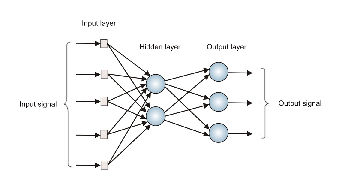
\includegraphics[keepaspectratio=true, scale=2.1]{editaveis/images/mlp.eps}
        \caption{Representação de uma MLP.}
        Fonte : Adaptado de \url{http://goo.gl/ICaZBQ}
    \end{figure}


